\documentclass[a4paper,ngerman,11pt,chapterprefix=false,oneside,openright]{scrreprt}
\usepackage[utf8]{inputenc}
\usepackage[ngerman]{babel}
\usepackage[headings]{fullpage}
\newcommand\tab[1][1cm]{\hspace*{#1}}

%Grafikeinbindung
\usepackage[pdftex]{graphicx,xcolor}
\graphicspath{{./src/pics/}}
\usepackage{pgfplots}
\pgfplotsset{compat=1.16}
\usepackage{tikz}
\usetikzlibrary{plotmarks,shapes,arrows.meta,decorations.markings,patterns,calc}

%Units
\usepackage{siunitx}
\sisetup{locale = DE} 

%Kopfzeile
\usepackage{geometry}
\geometry{verbose,a4paper,tmargin=3.5cm,bmargin=2.5cm,lmargin=2.6cm,rmargin=2.6cm,headheight=40pt,headsep=1cm}
\usepackage[headsepline= 0.4pt]{scrlayer-scrpage}
\pagestyle{scrheadings}
\clearscrheadfoot
\ohead{  \normalfont \sffamily \bfseries \small Universität Stuttgart \\[2pt] Institut für Flugmechanik und Flugregelung  \\[8pt] \normalfont\sffamily\footnotesize{Prof. Dr.-Ing. Walter Fichter}\\[-37pt] }
\lohead{ 
\includegraphics[scale=0.4, trim= -0.0cm 0.05cm 0cm 0cm] {./src/pics/logo/ifrlogo.pdf} \vspace{0.05cm}}
\cfoot[\pagemark]{}

%Mathematikfunktionen
\usepackage{amsmath,amsfonts,amssymb}
\usepackage{mathtools}

% ToDo-Notes
\usepackage{todonotes}

% References
\usepackage[hidelinks]{hyperref}
\usepackage{cleveref}

% % Tabellen- und Abbildungspakete 
% Multirow in Tabellen:
% Ermöglicht das Verbinden von Zeilen in Tabellen
\usepackage{multirow}
% Für schöne Tabellen, bietet dicke/dünne Linien an
% mehr Tabelleneinstellungen ( \toprule / \midrule / \bottomrule)
\usepackage{booktabs}
\renewcommand{\arraystretch}{1.3}		% Erhöht den Zeilenabstand von Tabellen leicht (Ästhetik)
\setlength{\tabcolsep}{5pt}
% Beide Pakete werden für die Ausrichtung der Tabellenspalten benötigt
\usepackage{array}
% Für lange Tabellen
\usepackage{longtable}
\usepackage{tabularx}				% mehr Tabelleneinstellungen (z.B. Tabellen mit benutzerdefinierter Breite)
%\usepackage{tikz}					% Erstellen von Vektorgrafiken in LaTeX
\pgfplotsset{compat=1.16}			% Neuste Version des Pakets aufrufen 
\pgfplotsset{plot coordinates/math parser=false} % (benötigt von matlab2tikz)
\newlength\fwidth					% Breite einer Matlab-Figure bestimmen mit \setlength\fwidth{}
\newlength\fheight					% Höhe einer Matlab-Figure bestimmen mit \setlength\fheight{}
% Darstellung für Caption
\usepackage[font=small,labelfont=bf,labelsep=endash,format=plain]{caption}

\makeindex
  
%==================================================================
 %==================================================================
 % Metadaten der Arbeit
 %
 % Titel
 \newcommand{\ifrtitleOne}{Systemidentifikation: }
 \newcommand{\ifrtitleTwo}{Schätzung der Parameter flugmechanischer Modelle aus Flugmessdaten}
 % Author
  \newcommand{\ifrauthor}{Calvin Ebert\\Adam Ghribi\\Florian Gschwandtner\\Fabrizio Turco}
 %
 %=================================================================== 
 %==================================================================
  

%Beispieltext
\usepackage{blindtext}

\begin{document}
%Titlepage
%********************************
% Titelseite
%********************************
\section*{
\pagenumbering{gobble}
\ohead{  \normalfont \sffamily \bfseries \small Universität Stuttgart \\[2pt] 
Institut für Flugmechanik und Flugregelung  \\[8pt] 
\normalfont\sffamily\footnotesize{Prof. Dr.-Ing. Walter Fichter}\\[-37pt] }
\lohead{ 
\includegraphics[scale=0.4, trim= -0.0cm 0.05cm 0cm 0cm] 
{./src/pics/logo/ifrlogo.pdf} \vspace{0.05cm}}
\vspace{4.5cm}
{\LARGE \\ 
Aerobotics-Seminar  \\
Moonshot-Aufgabe   \vspace{1.5cm}\\ 
\ifrtitleOne \\
\huge \ifrtitleTwo \\
\vspace{4.3cm} 
} 
{\normalsize
Autoren: Gruppe 02\\ 
\ifrauthor \vspace{1cm}\\
Datum: 06.08.2021
}
}

\listoftodos
\thispagestyle{empty}

%Table of contents
\tableofcontents
\pagenumbering{arabic} 

%Chapters
\chapter{Einleitung}

Die vorliegende Arbeit wurde im Rahmen des Aerobotics-Seminars im Sommersemester 2021 an der Universität Stuttgart verfasst. 
Ziel des Projekts war die Identifikation der Parameter eines linearisierten Modells der Längsbewegung aus vorliegenden 
Flugmessdaten eines 1:3-Modells des Flugzeugs \textit{e-Genius}. Für die Seitenbewegung wurde ebenfalls eine 
Systemidentifikation durchgeführt, aus Gründen der Übersichtlichkeit und Kürze wird diese aber in der Ausarbeitung 
ausgelassen.\par
Es werden Verfahren im Zeit- und im Frequenzbereich verwendet, um die Ergebnisse abschließend vergleichen zu können. Genauer 
handelt es sich dabei im Zeitbereich um die \textit{Least Squares}-Methode sowie die Matrix-LSQ-Methode. Im Frequenzbereich 
wird die \textit{Output Error}-Methode in Verbindung mit einem \textit{Newton-Raphson}-Algorithmus verwendet.\\

Linearisierte Modelle spielen eine wichtige Rolle in der Regelungstechnik: Mit ihnen lässt sich eine lineare Regelung um 
einen stationären Arbeits- bzw. Trimmpunkt entwickeln. Eine Schwierigkeit besteht dabei aber immer wieder darin, die 
Regelstrecke mit dem Modell ausreichend genau zu beschreiben. Hier kommt die Systemidentifikation ins Spiel: Sie hat zum Ziel 
aus gegebenen Flugmessdaten die Parameter des definierten Modells bestmöglich abzuschätzen.


\chapter{Modelle}

Im folgenden Abschnitt werden die der durchgeführten Systemidentifikationen 
zugrundeliegenden Modelle beschrieben, deren beiwerte zu bestimmen sind. Es 
handelt sich dabei um die bekannten linearisierten Modelle der Längs- und 
Seitenbewegung mit den folgenden Annahmen \cite{Fichter2009}:
\begin{itemize}
	\item Linearisierung um den symmetrischen Horizontalflug ($ \gamma_0=0 $)
	\item kein Auftrieb durch Nickrate ($ Z_q=0 $)
	\item keine Querkräfte durch Roll- oder Gierdrehrate ($ Y_p=Y_r=0 $)
	\item keine Querkraft durch Querruder ($ Y_\xi $)
	\item kein Wind ($ \Delta\gamma = \Delta\theta-\Delta\alpha $)
	\item horizontal eingebautes Triebwerk ($ i_F=0 $)
\end{itemize} 
Die Dynamiken können deshalb entkoppelt behandelt werden. %\cite{Vorlesung2}

\section{Längsbewegung}
Der Zustand der Längsbewegung setzt sich zusammen aus dem Anstellwinkel $ 
\alpha $, der Nickrate $ q $, der Anströmgeschwindigkeit $ V_A $ und dem 
Bahnwinkel $ \gamma $. Die zugehörigen Steuerungen umfassen den 
Höhenruderausschlag $ \eta $ und den Schubdrosselgrad $ \delta_F $. Bis auf die 
Nickrate werden alle Größen als Abweichungen (Delta-Größen) vom jeweiligen 
Trimmpunkt (gekennzeichnet durch den Index "$ _0 $") beschrieben. Es ergibt sich folgendes 
Modell \cite{Fichter2009}:

\begin{equation}\label{eq:laengsbewegung}
	\begin{pmatrix}
		\Delta \dot \alpha\\
		\dot q\\
		\Delta \dot V_A\\
		\Delta \dot \gamma
	\end{pmatrix} = 
	\begin{pmatrix}
		\frac{Z_\alpha}{V_0} & 1 & \frac{Z_V}{V_0} & 0\\
		M_\alpha & M_q & M_V & 0\\
		X_\alpha & 0 & X_V & -g\\
		-\frac{Z_\alpha}{V_0} & 0 & -\frac{Z_V}{V_0} & 0\\
	\end{pmatrix} \cdot
	\begin{pmatrix}
		\Delta \alpha\\
		q\\
		\Delta V_A\\
		\Delta \gamma
	\end{pmatrix} + 
	\begin{pmatrix}
		\frac{Z_\eta}{V_0} & -\frac{X_{\delta F}}{V_0} \sin{(\alpha_0)}\\
		M_\eta & M_{\delta F}\\
		X_\eta & X_{\delta F} \cos{(\alpha_0)}\\
		-\frac{Z_\eta}{V_0} & \frac{X_{\delta F}}{V_0} \sin{(\alpha_0)}\\
	\end{pmatrix}\cdot
	\begin{pmatrix}
		\Delta \eta\\
		\Delta \delta_F\\
	\end{pmatrix}
\end{equation}

\section{Seitenbewegung}
Das Modell der Seitenbewegung wird mit dem absoluten Zustand aufgestellt:

\begin{equation}\label{eq:seitenbewegung}
	\begin{pmatrix}
		\dot{r}\\
		\dot{\beta}\\
		\dot{p}\\
		\dot{\phi}
	\end{pmatrix} = 
	\begin{pmatrix}
		N_r & N_\beta             & N_p & 0\\
		-1  & \frac{Y_\zeta}{V_0} & 0   & \frac{g}{V_0}\\
		L_r & L_\beta             & L_p & 0\\
		0   & 0                   & 1   & 0\\
	\end{pmatrix} \cdot
	\begin{pmatrix}
		\dot{r}\\
		\dot{\beta}\\
		\dot{p}\\
		\dot{\phi}
	\end{pmatrix} + 
	\begin{pmatrix}
		N_\xi & N_\zeta\\
		0 & \frac{Y_\zeta}{V_0}\\
		L_\xi & L_\zeta\\
		0 & 0\\
	\end{pmatrix}\cdot
	\begin{pmatrix}
		\xi\\
		\zeta
	\end{pmatrix}
\end{equation}


\chapter{Vorbereitung der Daten}
Aus den Flugversuchen des e-Genius 1:3 liegt eine Fülle von Messdaten in verschiedenen .csv-Dateien vor. Im folgenden Kapitel 
wird erklärt, wie diese vorbereitet werden, um sie für die anschließende Systemidentifikation zu verwenden.



\section{Ermittlung der relevanten Signale} % Fabrizio
%\todo[inline]{Abschnitt "Ermittlung der relevanten Signale" schreiben}
Für die weitere Verarbeitung ist es zunächst nötig, aus den gegebenen Messdaten die relevanten Signalverläufe auszuwählen 
bzw. zu berechnen. Die meisten Zustandsgrößen können direkt aus den Messdaten verwendet werden, einzig der Bahnwinkel $ 
\gamma $ muss explizit berechnet werden. Die Bestimmung über die Beziehung $ \gamma=\theta-\alpha $ liefert dabei aufgrund 
eines unplausiblen Verlaufs des Nickwinkels $ \theta $ kein sinnvolles Ergebnis.\footnote{Berechnet man den Bahnwinkel auf 
diese Weise, nimmt er genau wie der Nickwinkel nie Werte kleiner 0 an. Lediglich der Anstellwinkel bewegt sich sowohl im 
positiven als auch im negativen Bereich.} Stattdessen wird der Bahnwinkel mit \cref{eq:gammaCalculation} über die 
geodätischen Geschwindigkeiten in $ z $- und $ x $-Richtung berechnet.

\begin{equation}
	\gamma = \arcsin{\left( \frac{V_z}{V_x} \right)}
	\label{eq:gammaCalculation}
\end{equation}

\cref{tab:messgroessen} zeigt eine Übersicht über die verwendeten Messsignale aus den Originaldateien. Zu beachten ist, dass 
in den Originaldaten für das Höhenruder jeweils ein eigenes Signal für das linke sowie das rechte 
Ruder vorlieg, im Falle es Querruders sogar zwei je Seite. Im betrachteten Bereich sind diese Signale jedoch zu jedem 
Zeitpunkt  gleich, weshalb die Verwendung eines Verlaufs je Steuerruder ausreicht.

\begin{table}[h!]
	\centering
	\caption{Übersicht über die verwendeten Messgrößen}
	\label{tab:messgroessen}
	\begin{tabular}{@{} cll @{}} 
		\toprule
		\multicolumn{3}{c}{Längsbewegung}\\
		\midrule
		Größe 	&Messsignal &Datei\\
		\midrule
		$ \alpha $	&Alpha &vectoflow\_airdata\\
		$ q $	&pitchspeed &vehicle\_attitude\\
		$ V_A $	&VMag &vectoflow\_airdata\\
		$ \gamma $ &vx, vz &vehicle\_local\_position\\
		$ \eta $ &elevator\_l &actuator\_controls\\
		$ \delta_F $ &thrust &actuator\_controls\\
		\bottomrule
	\end{tabular}
	\begin{tabular}{@{} cll @{}} 
		\toprule
		\multicolumn{3}{c}{Seitenbewegung}\\
		\midrule
		Größe 	&Messsignal &Datei\\
		\midrule
		$ r $	&yawspeed &vehicle\_attitude\\
		$ \beta $	&Beta &vectoflow\_airdata\\
		$ p $	&rollspeed &vehicle\_attitude\\
		$ \phi $ &Phi &vectoflow\_airdata\\
		$ \xi $ &aileron\_inner\_l &actuator\_controls\\
		$ \zeta $ &rudder &actuator\_controls\\
		\bottomrule
	\end{tabular}
\end{table}

Die vorliegenden Messdaten umfassen einen großen Zeitbereich von Start bis Landung. Für die Systemidentifikation wurde nur 
der Abschnitt berücksichtigt, in dem das Flugzeug Platzrunden fliegt. Dies entspricht im originalen Datensatz in etwa der 
Zeit zwischen $ \SI{910}{\second} $ und $ \SI{2225}{\second} $. \cref{fig:flug} zeigt den Flug und den entsprechenden 
Ausschnitt.

\begin{figure}[h!]
	\centering
	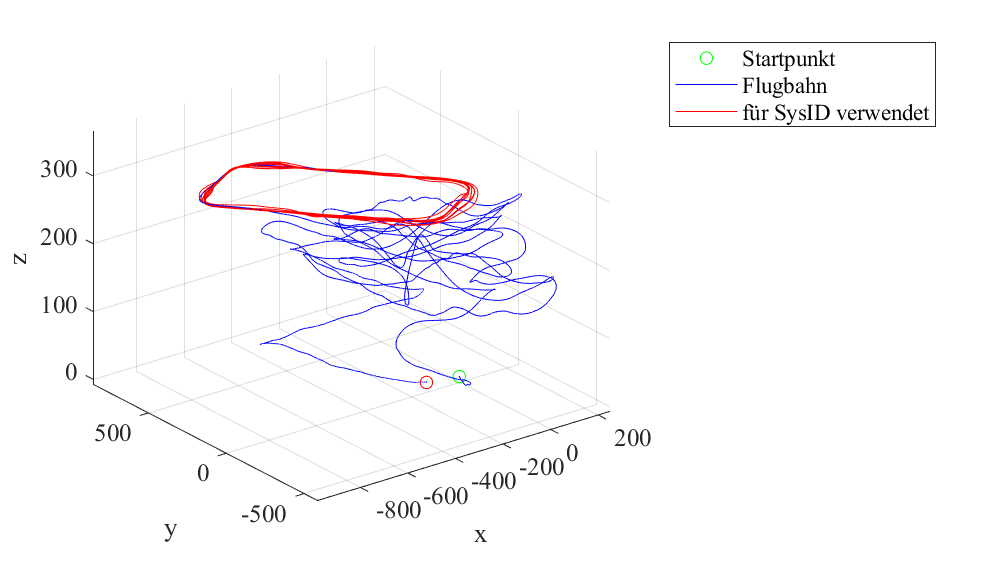
\includegraphics[width=0.9\linewidth]{flug.png}
	\caption{Visualisierung der Flugbahn}
	\label{fig:flug}
\end{figure}

\section{Trimmpunkt} % Fabrizio
In \cref{fig:trimmpunkte} ist beispielhaft der zeitliche Verlauf der Anströmgeschwindigkeit dargestellt. Es zeigen sich 
insgesamt acht stationären Bereiche, die als Trimmpunkt für eine Modellierung dienen könnten. In den nachfolgenden 
Systemidentifikationen soll jeweils der erste Punkt (TP 1) als Grundlage dienen. Dazu werden alle Zustands- und Steuergrößen 
über den Bereich TP 1 gemittelt und diese Mittelwerte als Trimmwerte $ x_0 $ und $ u_0 $ verwendet. Damit lassen sich die 
Abweichungen vom Trimmpunkt berechnen:
\begin{equation}
	\begin{split}
		\Delta x(t) &= x(t)-x_0\\
		\Delta u(t) &= u(t)-u_0
	\end{split}
\end{equation}

Eine Ausnahme bilden hier die Drehraten $ p $, $ q $ und $ r $, bei denen keine Differenz zum Trimmwert gebildet werden muss.


\begin{figure}[h!]
	\centering
	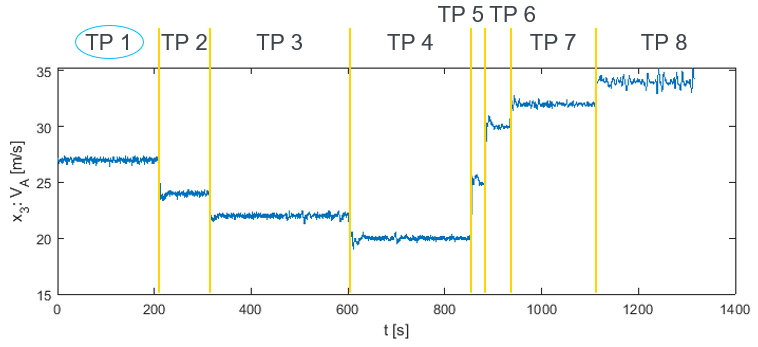
\includegraphics[width=0.9\linewidth]{trimmpunkte.png}
	\caption{zeitlicher Verlauf der Anströmgeschwindigkeit mit den stationären Bereichen}
	\label{fig:trimmpunkte}
\end{figure}




\section{Interpolation} %Florian
Die Rohdaten werden von mehreren Sensoren mit unterschiedlichen Abtastraten geliefert. Da die Identifikationsalgorithmen die 
Werte zu diskreten Zeitpunkten benötigen, ist es notwendig, einen einheitlichen Zeitvektor mit zugehörigen Eingangs- und 
Zustandsvektoren zu generieren. Außerdem wird eine konstante Schrittweite gefordert.

Die Abtastrate dieses Zeitvektors ist wichtig, da die Dimension des Optimierungsproblems und damit der 
Rechenaufwand mit feinerer Diskretisierung steigt (im Zeitbereich). In dieser Arbeit wird der Zeitvektor des 


\begin{figure}[h!]
	\centering
	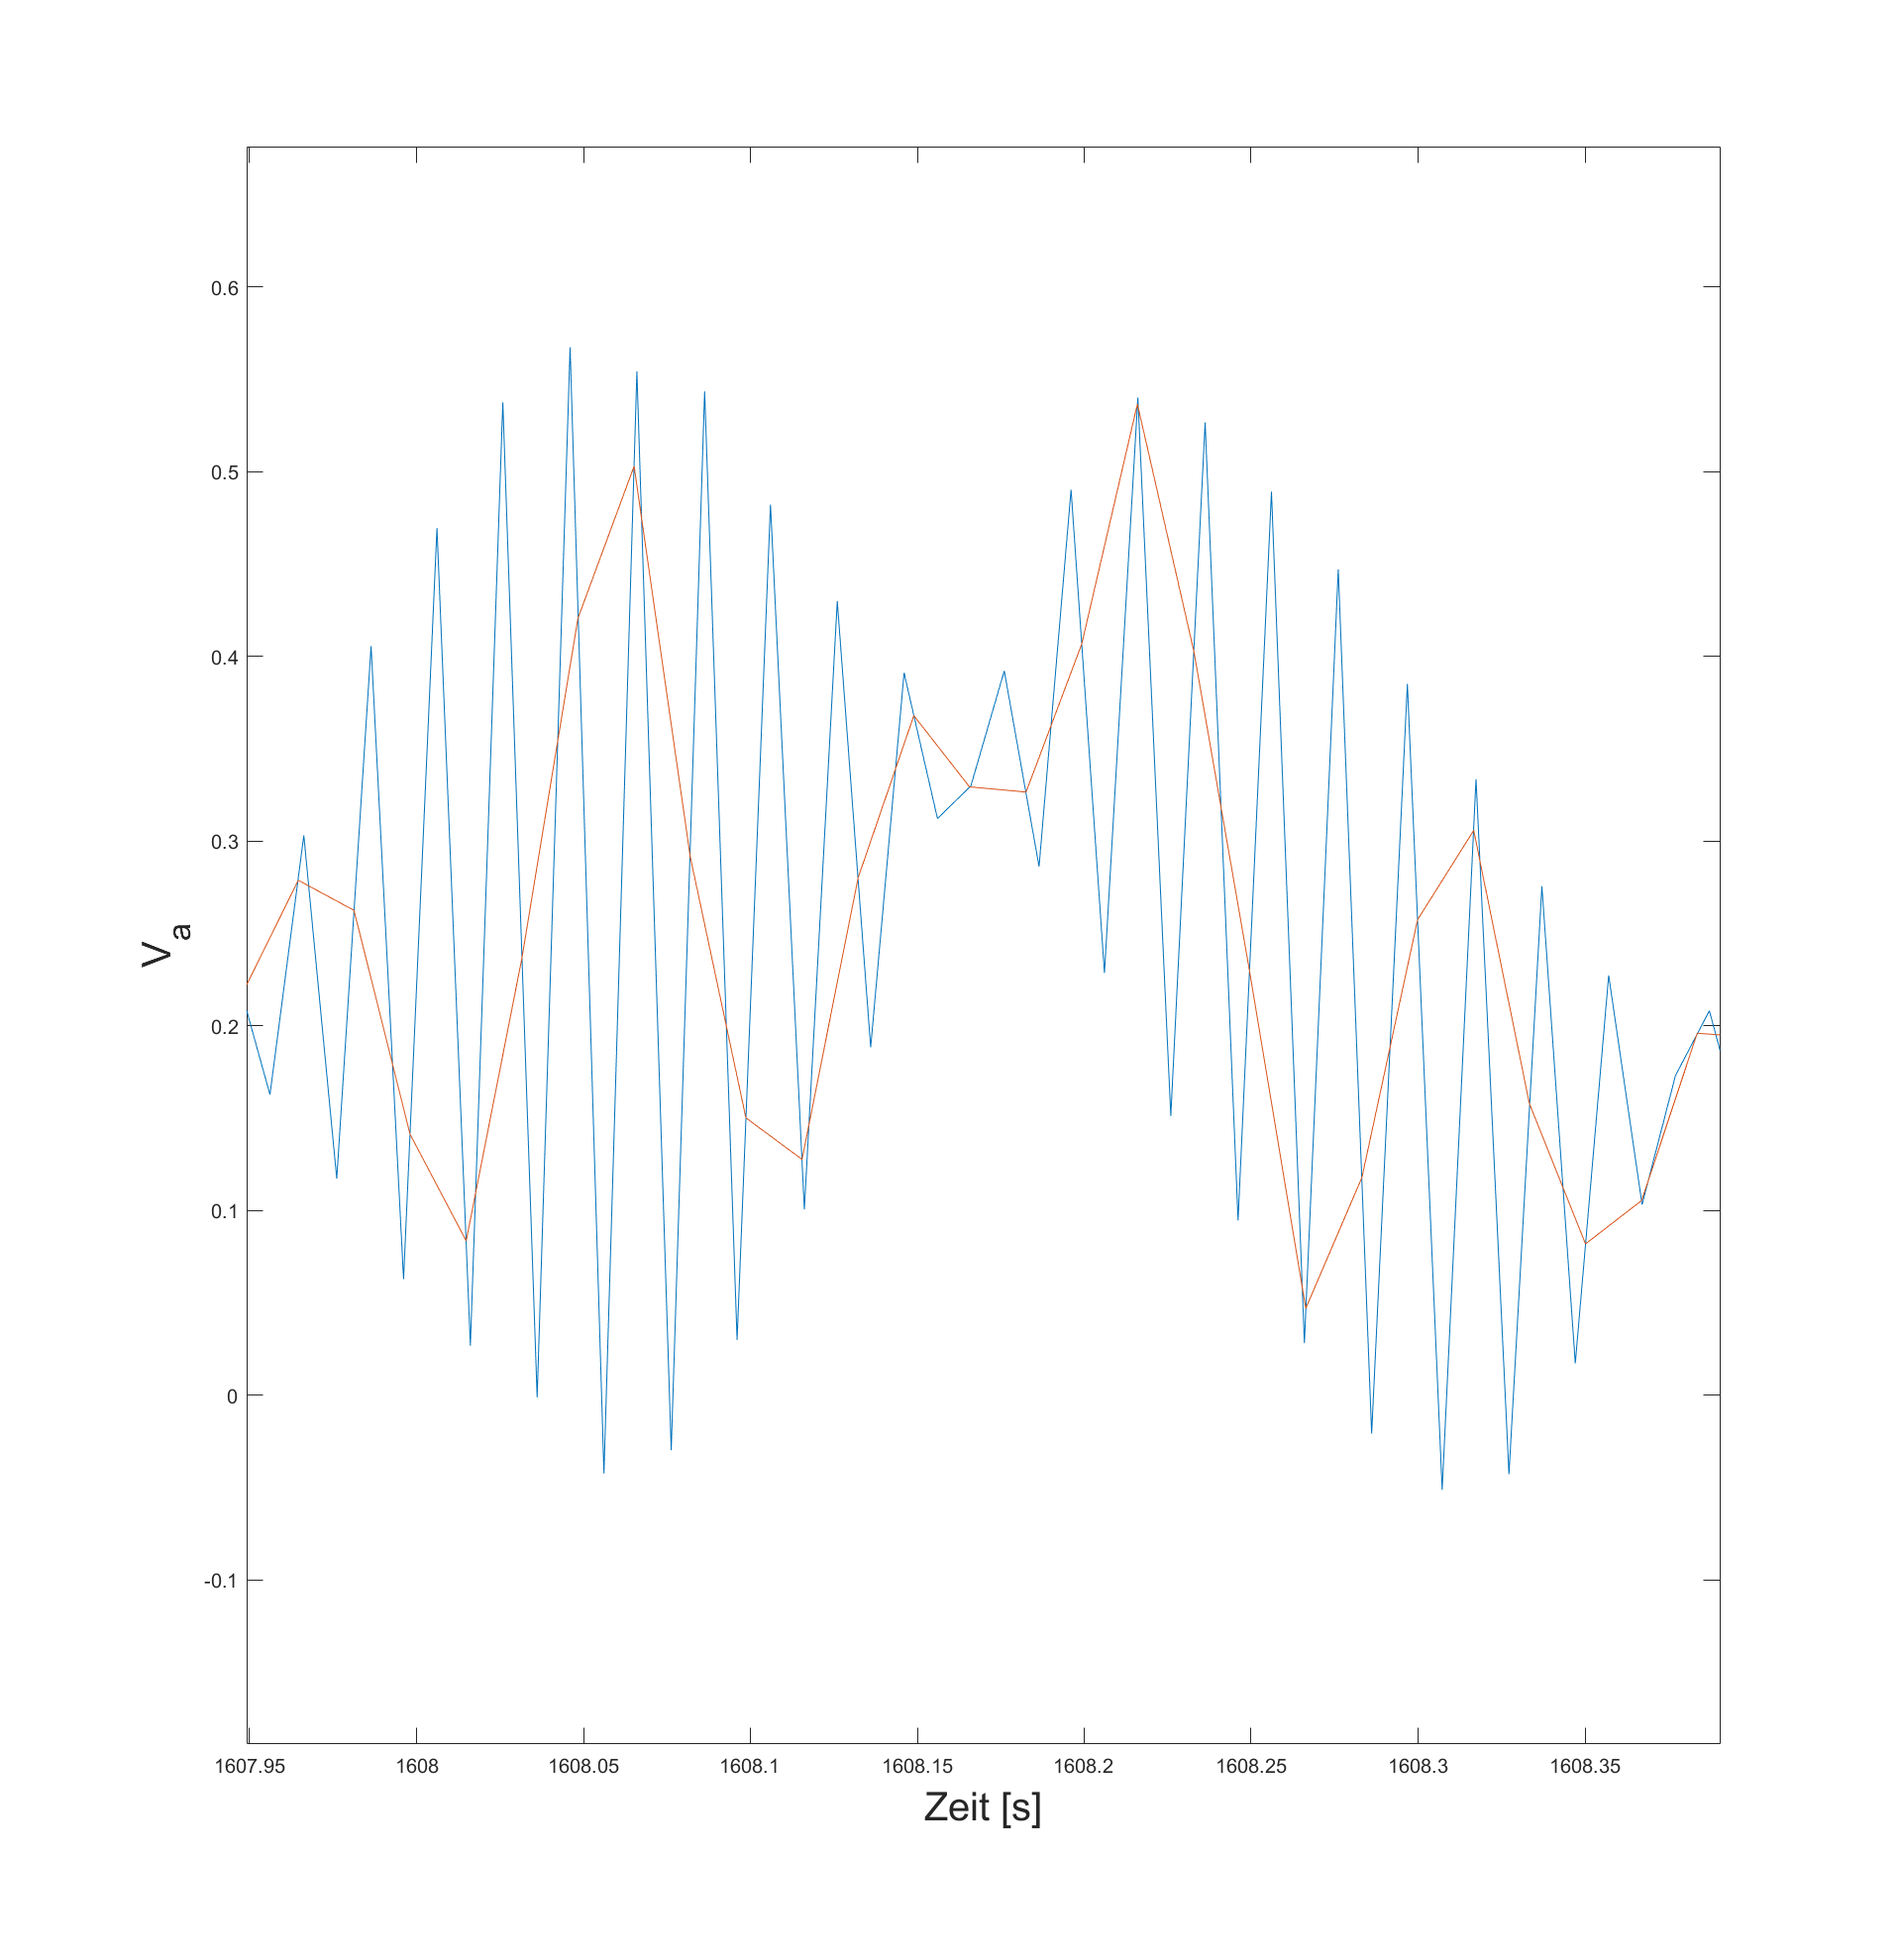
\includegraphics[width=0.7\linewidth]{beispielInterpolation.png}
	\caption{Beispiel Interpolation}
	\label{fig:interpBsp}
\end{figure}

%fkt interp1

\section{Filterung} %Florian

Verrauschte Messdaten stellen für die Systemidentifikation eine Herausforderung dar. Numerische Ableitungen aus verrauschten Daten liefern in vielen Fällen keine sinnvolle Aussage. Neben aufwändigeren Ableitungsregeln bietet sich eine vorangehende Filterung der Daten an.

Das Vorwärts-Rückwärtsfilter bietet den Vorteil, dass keine Phasenverschiebung 
auftritt. Gerade wenn nur einzelne Signalteile gefiltert werden, beispielsweise 
nur der Eingang, ist diese Eigenschaft unerlässlich. Der Nachteil ist, dass das 
Filter nicht in Echtzeit verwendet werden kann, da immer die vollständige 
Datenreihe vorliegen muss. Für eine Systemidentifikation ist dies jedoch keine 
praktische Einschränkung.

In \cref{fig:filterBsp} sind die Auswirkungen einer reinen Vorwärts- und einer Vorwärts-Rückwärtsfilterung auf die Phase 
gut zu sehen.

\begin{figure}[h!]
	\centering
	\includegraphics[width=0.7\linewidth]{beispielFilterung.png}
	\caption{Beispiel Filterung}
	\label{fig:filterBsp}
\end{figure}


\subsection{Ablauf}

Für das Filter wird eine Übertragungsfunktion $f(s)$ auf die Messdaten vorwärts 
angewandt, die Messdaten umgekehrt und die selbe Übertragungsfunktion noch 
einmal verwendet. In Matlab ist dies in der Funktion \textit{filtfilt()} 
bereits implementiert. 

\subsection{Wahl der Filterübertragungsfunktion}

Es wurde ein quadriertes PT2-Glied gewählt, da so die Eckfrequenz direkt eingestellt werden kann. Die Eckfrequenz wurde zu $ 
\SI{20}{\hertz} $ gewählt, damit das Rauschen unterdrückt wird, aber keine Information verloren geht.

Mit

\begin{equation}
	\omega_{filt} = 2 \cdot \pi \cdot f_{eck} = 2 \cdot \pi \cdot \SI{20}{\hertz}
\end{equation}

%\todo{gewählte Eckfrequenz nennen}

und der Dämpfung

\begin{equation}
	\zeta_{filt} = \frac{1}{\sqrt{2}}
\end{equation}

ergibt sich die Übertragungsfunktion zu:

\begin{equation} \label{eq:filter}
	f(s) = \left(\frac{\omega_{filt}^2}{s^2+2 \cdot \zeta_{filt} \cdot \omega_{filt} +\omega_{filt}^2}\right)^2
\end{equation}

Im Bodediagramm, \cref{fig:bodeplot}, sind Amplituden- und Frequenzgang der Filterfunktion zu sehen.

\begin{figure}[h!]
	\centering
	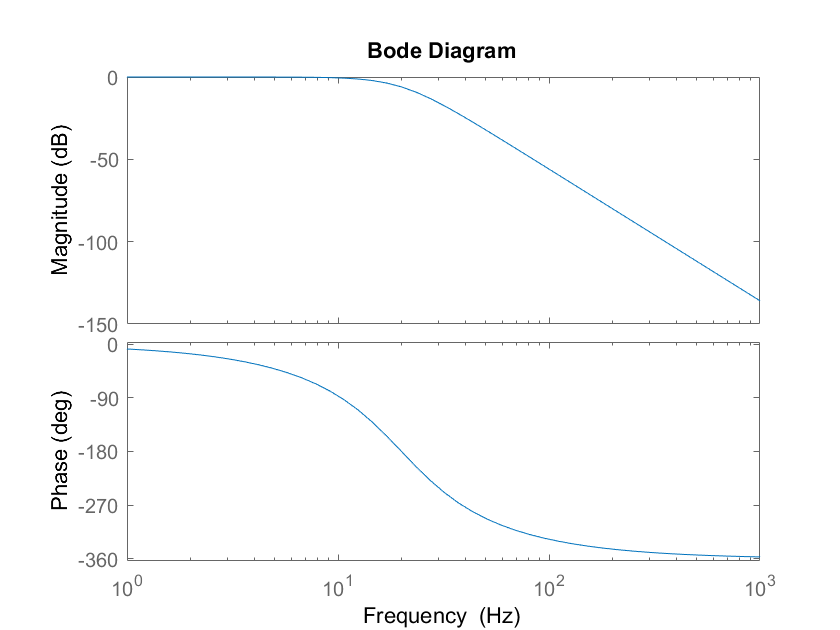
\includegraphics[width=0.7\linewidth]{bodeplot.png}
	\caption{Bodediagramm der Filterfunktion aus \cref{eq:filter}}
	\label{fig:bodeplot}
\end{figure}
\chapter{Systemidentifikation im Zeitbereich}
Systemidentifikation im Zeitbereich heißt, ein Modell und den zugehörigen Parametersatz zu finden, welches den zeitlichen Verlauf möglichst gut approximiert. Grundlegend ist hier zwischen der Systemidentifikation und der Parameteridentifikation zu unterscheiden. Systemidentifikation bedeutet, dass auch das Modell als unbekannt angenommen wird und die gesamte Struktur aus den Messdaten geschätzt wird, wie es hier mit der Matrix LSQ . Bei der Parameteridentifikation hingegen ist ein flugmechanisches Modell bekannt, in dem Parameter gesucht werden.

\section{\textit{Least Squares}-Methode}
In diesem Kapitel wird die Methode der kleinsten Fehlerquadrate (\textit{Least Squares}, LSQ) vorgestellt.
Eine der Kernaufgaben vieler Ingenieure besteht darin, einen belastbaren Zusammenhang zwischen gemessenen Werten zu finden. 
Diese Zusammenhänge können näherungsweise durch folgendes lineares Modell beschrieben werden:  
\begin{equation}
    z = H\cdot x+v 
\end{equation}
mit 
\begin{align}
	\begin{split}
		\text{Messvektor: } &\dim{(z)} = m\times 1\\
		\text{bekannte Matrix: } &\dim{(H)} = m\times n\\
		\text{unbekannter Rauschterm: } &\dim{(v)} = m\times1\\
		\text{unbekannter Parametervektor: } &\dim{(x)} = n\times 1
		\nonumber
	\end{split}
\end{align}

Die LSQ-Methode kann beispielsweise verwendet werden, um die Schätzung von Modellparametern im Rahmen der 
Systemidentifikation durchzuführen. Gesucht ist dabei ein Schätzwert $\hat{x}$ für den Parametervektor. Der Restfehlervektor 
$e$ lautet:
\begin{equation}
    e = z - H\cdot \hat{x} \\
\end{equation}

Die Idee besteht darin, einen Wert von $\hat{x}$ zu finden, der die Norm des quadrierten Restfehlervektors minimiert. Das 
quadratische Zielfunktional $J$ ist gegeben durch: 
\begin{align}
   \begin{split}
     J &= \frac{1}{2} \cdot e^{T} \cdot e \\
     &= \frac{1}{2} \cdot {(z- H\hat{x})}^{T}\cdot(z- H\hat{x}) \\
     &= \frac{1}{2} \cdot (z^{T} -{\hat{x}}^{T}H^{T})\cdot(z- H\hat{x}) \\
     &= \frac{1}{2} \cdot z^{T}z - z^{T}H\hat{x} + \frac{1}{2}\cdot {\hat{x}}^{T}A\hat{x}  \\
   \end{split}
\end{align}
mit $A = H^{T}H$. Die Lösung des Minimierungsproblems lautet dann:
\begin{equation}
    \hat{x}= {(H^{T} H)}^{-1} \cdot H^{T} z 
\end{equation}


\subsection{Schätzung der Parameter mit dem LSQ-Verfahren} 

Die Zustandsraumdarstellung \eqref{eq:laengsbewegung} liefert folgende Gleichungen: 

\begin{align}
	\Delta\dot \alpha-q &=  \frac{Z_{\alpha}\Delta\alpha}{V_0} + \frac{Z_{\nu}\Delta V_{A}}{V_0} + 
	\frac{Z_{\eta}\Delta\eta}{V_0} - \frac{X_{\delta_F}\sin{(\alpha_0)}\cdot\Delta\delta_F}{V_0}\\
	\dot q &= M_{\alpha}\Delta\alpha + M_q q + M_{\nu}\Delta V_A + M_{\eta}\Delta\eta + M{\delta_F}\Delta\delta_F\\
	\Delta\dot V_A &= X_{\alpha}\Delta\alpha +  X_{\nu}\Delta V_A + X_{\eta}\Delta\eta + 
	X_{\delta_F}\cos{(\alpha_0)}\cdot\Delta\delta_F \\
	\Delta \dot \gamma &= \frac{- Z_{\alpha}\Delta\alpha}{V_0} + \frac{- Z_{\nu}\Delta V_{A}}{V_0} + 
	\frac{-Z_{\eta}\Delta\eta}{V_0} + \frac{X_{\delta F}\sin{(\alpha_0)}\cdot\Delta\delta_F}{V_0}
\end{align}
	
Diese können zu einem linearen Gleichungssystem umgeformt werden: 
\begin{equation}
    z_{L}= H_{L}\cdot x + v
\end{equation}

Die einzelnen Vektoren und Matrizen lauten:
\setcounter{MaxMatrixCols}{15}
\begin{equation}
	z_{L} = (\Delta\dot \alpha-q \;\; \dot q \;\; \Delta\dot V_A)^T
\end{equation}

\begin{equation}
	 H_{L} = \begin{pmatrix}
		0&0&0& \frac{-\sin{(\alpha_0)}\cdot\Delta\delta_F}{V_0} & \frac{\Delta\alpha}{V_0}& \frac{\Delta V_A}{V_0} & 
		\frac{\Delta\eta}{V_0} &0&0&0&0&0   \\
		0&0&0&0&0&0&0 &\Delta\alpha & q & \Delta V_A & \Delta\eta & \Delta\delta_F \\
		\Delta\alpha &  \Delta V_A & \Delta\eta & \cos{(\alpha_0)}\cdot\Delta\delta_F &0&0&0&0&0&0&0&0 
	\end{pmatrix}
\end{equation}

\begin{equation}
	x = (X_{\alpha}\; 
	X_{\nu}\;
	X_{\eta}\;
	X_{\delta_F}\; 
	Z_{\alpha}\; 
	Z_{\nu}\;
	Z_{\eta}\;
	M_{\alpha}\;
	M_{q}\;
	M_{\nu}\;
	M_{\eta}\;
	M_{\delta_F})^T \\
\end{equation}  
Wie schon in dem letzten Abschnitt erwähnt, wird es nach einem geschätzten Paramertervektor $\hat{x}$ gesucht, der die Norm des quadrierten Restfehlervektors $ e = z - H\cdot \hat{x}$ minimiert. Die Lösung ist laut (4.4)
\begin{equation}
    \hat{x}= {({H_L}^{T} {H_L})}^{-1} \cdot {H_L}^{T} z_L 
\end{equation}


\section{Schätzung mit Matrix-LSQ}

Bei der Matrix-LSQ Methode wird, im Gegensatz zur klassischen LSQ Schätzung, sowohl die Systemmatrix \textbf{A} wie auch die Eingangsmatrix \textbf{B} als unbekannt angesehen. Es handelt sich somit um eine Systemidentifikation im eigentlichen Sinn, da keine flugmechanischen Modelle verwendet werden.

\subsection{Modellgleichung}

Messdaten der Eingänge $\textbf{u}$, des Zustands  $\textbf{x}$ und der Zustandsableitung $\dot{\textbf{x}}$ werden in die Form von Gl. \ref{eq:matrixLSQ} gebracht. 

\begin{equation}
    \underbrace{\begin{pmatrix}
        \dot{x}_1^T \\
        . \\
        . \\
        \dot{x}_n^T 
    \end{pmatrix}}_{\textbf{z}} =
    \underbrace{\begin{pmatrix}
        x_{1}^T& u_{1}^T \\
        . & .  \\
        . & .  \\
        x_{n}^T & u_{n}^T \\
    \end{pmatrix}}_{\textbf{H}}
    \underbrace{\begin{pmatrix}
        \textbf{A}^T \\
        \textbf{B}^T
    \end{pmatrix}}_{\hat{\textbf{x}}} +
    \begin{pmatrix}
        v_1^T \\
        . \\
        . \\
        v_n^T
    \end{pmatrix}
\end{equation}\label{eq:matrixLSQ}

\begin{tabular}[\textwidth]{l l}

$\textbf{z}$ & Messmatrix \\
$\textbf{H}$ & Modellmatrix \\
$\hat{\textbf{x}}$ & Schätzwertmatrix \\
$\textbf{v}$ & Störgrößenmatrix \\
$n$ & Anzahl der Zeitschritte \\
\end{tabular}

Die Dimension der Systemmatrix und der Eingangsmatrix werden von den Dimensionen von $\textbf{u}$,  $\textbf{x}$ und $\dot{\textbf{x}}$ vorgegeben. Hier liegt auch der Nachteil der Matrix-LSQ Methode. Es ist nicht möglich die einzelnen Parameter innerhalb der Matrizen zu beeinflussen oder Wertebereiche vorzugeben.


\subsection{Schätzgleichung}

Nach der Herleitung in \cite{Mandry2021} ergibt sich die Schätzgleichung zu:

\begin{equation*}
    \hat{\textbf{x}} = (\textbf{H}^T \textbf{H})^{-1}\textbf{H}^T\textbf{z}
\end{equation*}

Besonders hervorzuheben ist hier die Inversion der Matrix $\textbf{H}^T \textbf{H}$. Es handelt sich dabei um eine Matrix der Dimension (dim(\textbf{x})+dim(\textbf{u}))x(dim(\textbf{x})+dim(\textbf{u})). In dieser Arbeit bedeutet das konkret 6x6, womit der Rechenaufwand für die, für große Matrizen aufwändige, Inversion klein bleibt.
 
\section{Ergebnisse}
 
Anschließend werden die Ergebnisse in diesem Kapitel kurz vorgestellt.

Nach der Schätzung der Einträge der Matrizen $A$ und $B$ wird das Anfangswertproblem \eqref{eq:laengsbewegung} im gesamten 
Zeitintervall gelöst. Bei allen Simulationen sind die Filterparametern wie in \ref{section:filterung} gewählt.

In \cref{fig:Ergebnisse_zmlsq} wird die Lösung anhand des Matrix-LSQ-Verfahrens dargestellt. Die geschätzte Matrizen $A_L$ und $B_L$ lauten: 
\begin{equation}
 	A_L = \begin{pmatrix}
 		-0.1940 & 0.005 & -0.0002 & -0.0540 \\
 		-38.9899 & -12.8888 & 0.3632 & -4.2686 \\
 		-6.1506 & -0.1501 & -0.0589 & -5.0107 \\
 		0.4433 & 0.0427 & 0.0023 & 0.0818
 	\end{pmatrix} \;\;\; , \;\;\;
 	A = \begin{pmatrix}
		\frac{Z_\alpha}{V_0} & 1 & \frac{Z_V}{V_0} & 0\\
		M_\alpha & M_q & M_V & 0\\
		X_\alpha & 0 & X_V & -g\\
		-\frac{Z_\alpha}{V_0} & 0 & -\frac{Z_V}{V_0} & 0\\
	\end{pmatrix}
	\nonumber
\end{equation}

\begin{equation}
 	 B_L = \begin{pmatrix}
 		-0.0267 & -0.0164 \\ 
 		-26.1377 & -12.9651 \\
 		-0.7414 & 4.6092 \\
 		0.0477 & -0.1328
 	\end{pmatrix}  \;\;\; , \;\;\;
 	B= \begin{pmatrix}
		\frac{Z_\eta}{V_0} & -\frac{X_{\delta F}}{V_0} \sin{(\alpha_0)}\\
		M_\eta & M_{\delta F}\\
		X_\eta & X_{\delta F} \cos{(\alpha_0)}\\
		-\frac{Z_\eta}{V_0} & \frac{X_{\delta F}}{V_0} \sin{(\alpha_0)}\\
	\end{pmatrix}
 \nonumber
\end{equation}
Die Ergebnisse in \cref{fig:Ergebnisse_zmlsq} zeigen eine relativ präzise Approximation, das Modell liefert vor Allem für Anstellwinkel und Geschwindigkeit gute Ergebnisse. Auch die Ergebnisse für q und den Bahnwinkel sind sinnvoll, durch die wenig aussagekräftigen Messdaten aber schwer zu vergleichen. Allerdings weist das Ergebnis in flugmechanischer Hinsicht Abweichungen in System- und Eingangsmatrix auf. Der Betrag der Einträge der ersten und vierten Spalten von $A_L$ unterscheiden sich stark voneinander ($-0.1940$ und $0.4433$) und ($-0.0002$ und $0.0023$). Eine Starke Abweichung ist auch zwischen die vierten Spalten der Matrizen $A_L$ und $A$.  

%\todo{warum schlechte Ergebnisse? : Adam : ich weiß nicht warum?}
\begin{figure}[h!]
	\centering
	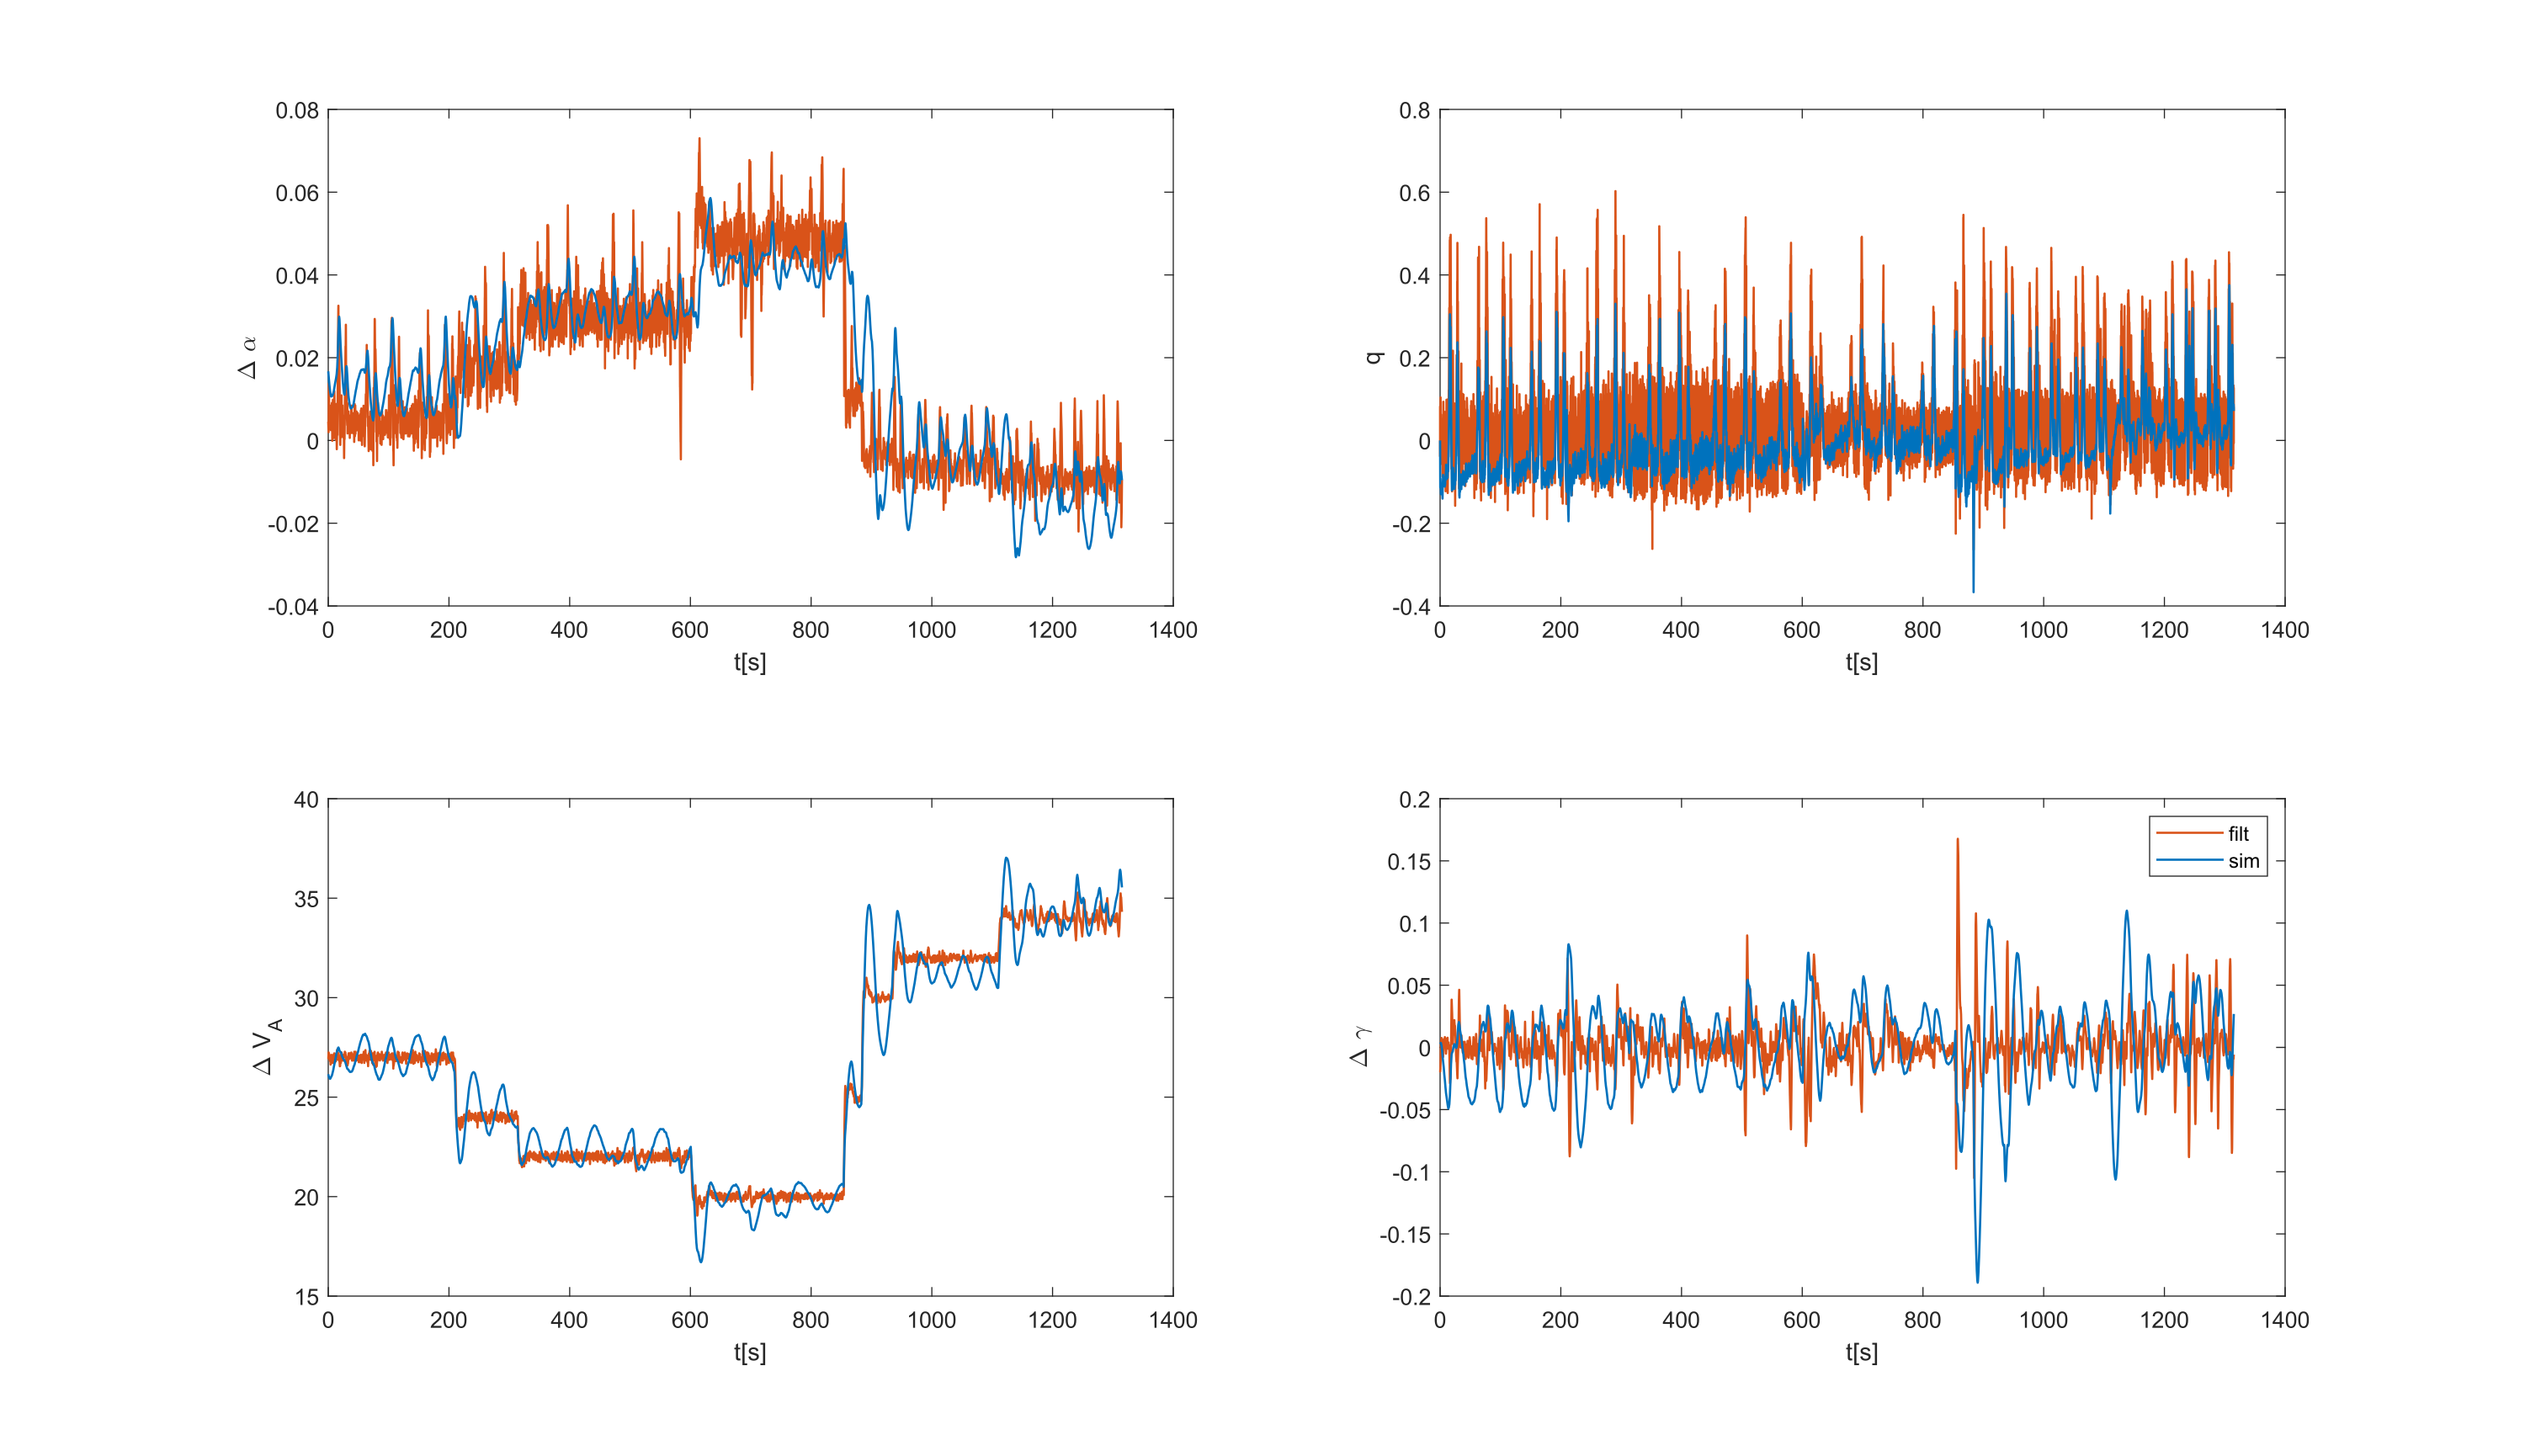
\includegraphics[trim=100 0 100 0,clip,width=1\linewidth]{LS.png}
	\caption{Ergebnisse anhand des Matrix-LSQ-Verfahrens}
    \label{fig:Ergebnisse_zmlsq}
\end{figure}

\cref{fig:Ergebnisse_zlsq} zeigt die Lösung anhand des LSQ-Verfahrens. Die Methode liefert kein sinnvolles Ergebnisse. Der Simulator kann keine stabilen Werten generieren.

 \begin{figure}[h!]
	\centering
	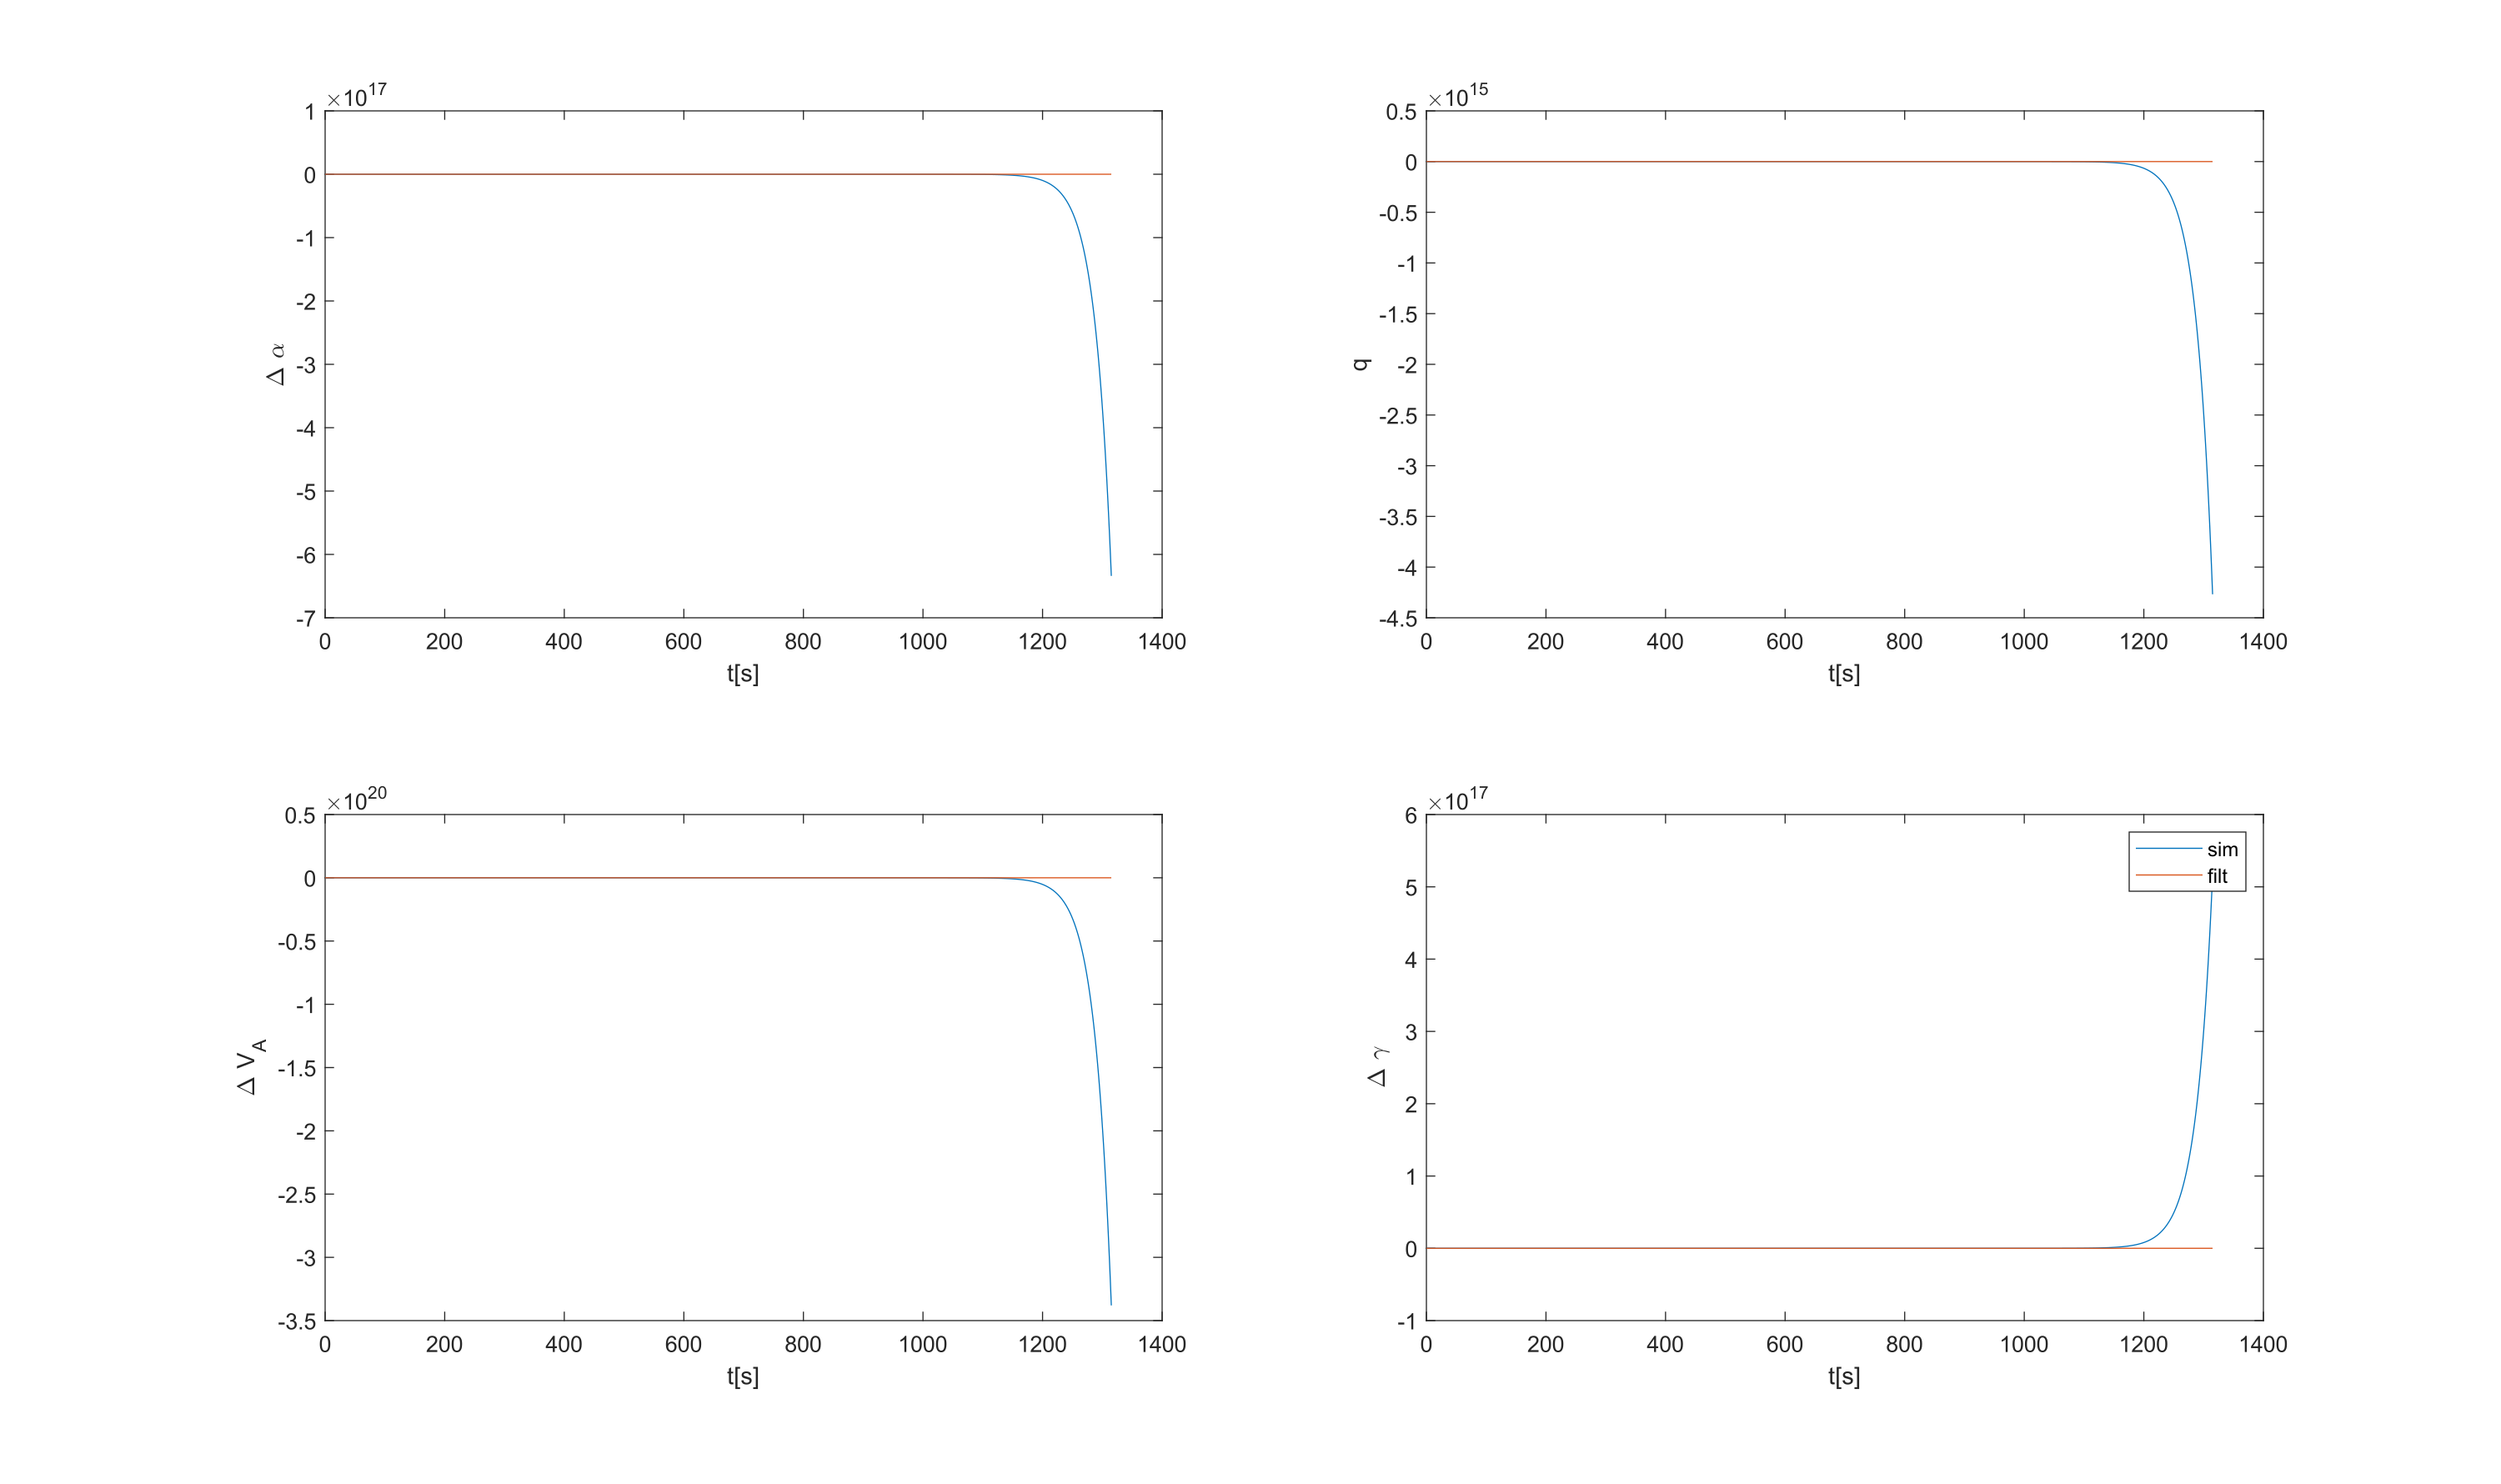
\includegraphics[trim=100 0 100 0,clip,width=1\linewidth]{LS_LSQ.png}
	\caption{Ergebnisse anhand des LSQ-Verfahrens}
     \label{fig:Ergebnisse_zlsq} 
\end{figure}


\section{Interpretation}

Die wesentliche Erkenntnis der Analyse im Zeitbereich ist, dass es nicht möglich ist die Parameter des linearen Modells für die Seitenbewegung so zu bestimmen, dass eine stabile Simulation möglich ist.

Eine Interpretation dafür ist, dass mithilfe der Matrix-LSQ Effekte übertragen werden, die vom linearen Modell vernachlässigt werden. Die in Kap. \ref{chapter:Modell} beschriebenen Vereinfachungen sind hier ein guter Ansatz. Besonders ist es möglich, dass der Wind und der Auftrieb durch die Nickrate eine relevante Rolle spielt. 
%Gerade die Elemente A[1,4] und A[2,4] sprechen dafür, weil durch diese der Bahnwinkel auf die Änderung des Anstellwinkels übertragen wird. 

Dass Element $\textbf{A}_L[1,4]$ nicht null ist spricht für einen Einfluss des Windes, weil somit $\Delta \gamma = \Delta \theta- \Delta \alpha$ nicht mehr gilt. Der Bahnwinkel hat somit einen Einfluss auf den Anstellwinkel.

Eine weitere Untersuchung und eine Betrachtung der Bedingungen beim Flugversuch sind hier notwendig, um eine fundierte Aussage zu treffen.

\chapter{Systemidentifikation im Frequenzbereich}

Neben der Systemidentifikation im Zeitbereich ist es möglich die Parameterschätzung auch im Frequenzbereich durchzuführen. 
Die Analyse im Frequenzbereich bringt einige Vorteile mit sich, die im weiteren Verlauf dieser Dokumentation genauer 
beleuchtet werden. Die Grundlage der Frequenzanalyse ist die Fouriertransformation der gemessenen Daten vom Zeitbereich in 
den Frequenzbereich. Ausgehend von den transformierten Messwerten wird im Folgenden genauer auf die Idee der 
Output-Error-Methode und auf den Algorithmus zur Lösung des Schätzproblems eingegangen. Zum Schluss werden die Ergebnisse 
bewertet und der Blick auf mögliche Verbesserungen und andere Methoden gerichtet.


\section{Fouriertransformation}  

\begin{align}
	j\omega_{k}\mathbf{\tilde{x}}(k)  &= \mathbf{A\tilde{x}}(k) + \mathbf{B\tilde{u}}(k) \nonumber \\
 	\mathbf{\tilde{y}}(k)             &= \mathbf{C\tilde{x}}(k) + \mathbf{D\tilde{u}}(k) = \mathbf{G}(k,\mathbf{\theta})\mathbf{\tilde{u}}(k) \nonumber \\
 	\text{mit }\mathbf{G}(k,\mathbf{\theta}) &= \mathbf{C}(j\omega\mathbf{I}-\mathbf{A})^{-1}\mathbf{B}+\mathbf{D}
	\label{eq:ZRD_Frequenzbereich}
\end{align}

\missingfigure{Bild von Fourier-Trafo}


\section{Output-Error-Methode}

Die Idee der Output-Error-Methode (OEM) liegt in der Art der Fehlerbetrachtung. Es wird dabei der Fehler, der durch die 
mathematische Modellbildung entsteht, vernachlässigt. Das dynamische System wird als deterministisch angenommen. 
Unsicherheiten entstehen nur durch fehlerhafte und verrauschte Messungen. Ausgangspunkt der OEM ist das transformierte 
Zustandsraummodell (\ref{eq:ZRD_Frequenzbereich}). Im vorliegenden Fall entspricht der Ausgangsvektor $\tilde{y}$ dem 
Zustandsvektor $\tilde{x}$. Die Matrizen $\mathbf{C}$ und $\mathbf{D}$ nehmen also folgende Gestalt an:

\begin{align}
	\mathbf{C} &= \mathbf{I} \nonumber \\
 	\mathbf{D} &= \mathbf{0}          
	\label{eq:CD}
\end{align}

Da der Zustandsvektor gleichzeitig der gemessene Zustand ist, kann der Output-Error folgendermaßen formuliert werden:

\begin{equation}
    \mathbf{\tilde{\nu}}(k,\mathbf{\theta}) = \mathbf{\tilde{z}}(k)-\mathbf{\tilde{y}}(k,\mathbf{\theta}) = \mathbf{\tilde{z}}(k)-\mathbf{G}(k,\mathbf{\theta})\mathbf{\tilde{u}}(k)  
	\label{eq:Output_Error}
\end{equation}

$\mathbf{\tilde{z}}$ entspricht dabei dem gemessenen Zustand, der durch Messrauschen aus dem übertragenen Zustand 
$\mathbf{\tilde{y}}$ entsteht. Der übertragene Zustand kann aus den Steuergrößen $\mathbf{\tilde{u}}$ durch Multiplikation 
mit der Übertragungsmatrix $\mathbf{G}(\mathbf{\theta)}$ berechnet werden. Die Übertagungsmatrix ist, wie in 
\cref{eq:ZRD_Frequenzbereich} gezeigt, abhängig vom zugrunde liegenden Modell und von den zu schätzenden Parametern 
$\mathbf{\theta}$. Diese sind die Einträge der Matrizen des Zustandsraummodells.   


\section{Ergebnisse}
\chapter{Zusammenfassung und Ausblick}\label{chapter:Zusammenfassung}
Abschließend lässt sich sagen, dass die Datenvorbereitung ein sehr wichtiger und auch zeitintensiver Teil der gesamten Arbeit 
war. Die richtigen Messsignale aus der Fülle an Originaldaten zu finden und auf Plausibilität zu prüfen legt den Grundstein 
für alle weiteren Schritte. Schwierig ist außerdem die Auswahl eines geeigneten Zeitbereichs zur Identifikation. 

Das LSQ-Verfahren im Zeitbereich lieferte keine sonderlich guten Ergebnisse. Deutlich bessere Approximationen der Messdaten 
ließen sich mit dem Matrix-LSQ-Verfahren erreichen. Dieses stellte sich als sehr schnell und vergleichsweise einfach in der 
Implementierung heraus. Aus flugmechanischer Sicht sind allerdings Einbußen in den bestimmten Parametern hinzunehmen, da sich 
keine Vorgaben bzgl. der bereits bekannten Einträge in der System- und Steuermatrix treffen lassen.

Es zeigte sich, dass der Flug in den Platzrunden weniger geeignet für eine Identifikatition im Frequenzbereich ist. Der 
Verlauf des Steuersignals ist hier von großer Relevanz, bestimmte Manöver, wie ein \textit{Frequency Sweep}, sollten hier zu 
deutlich besseren Ergebissen führen. Nichtsdestotrotz konnten bestimmte Zustandsgrößen angenähert werden. Der 
Implementierungsaufwand für die \textit{Output Error}-Methode ist deutlich höher verglichen mit den Zeitbereich-Verfahren; 
die symbolische Berechnung der sehr länglichen Ableitungen in Matlab ermöglichte überhaupt erst eine sinnvolle Anwendung.\\

An dieser Stelle sei erneut erwähnt, dass in der vorliegenden Arbeit lediglich der Platzrundenflug berücksichtigt wurde. In 
den restlichen Flugdaten steckt aber womöglich ebenso Potenzial zur Bestimmung des flugmechanischen Modells, vor allem, wenn 
sich noch passende Manöver (z.B. Anregung der Eigenschwingung des Flugzeugs) finden lassen. Als nächster Schritt bietet sich 
also eine genaue Untersuchung des bisher vernachlässigten Flugs an.

Möglichkeiten zur Verfeinerung und Optimierung der Identifikation selbst gibt es viele. An erster Stelle bietet sich eine 
Normalisierung der Signale an, d.h. eine Skalierung mit den Maximalwerten eines jeden Verlaufs, sodass die Werte danach in 
der gleichen Größenordnung liegen. Dies ist sonst nicht der Fall, die Geschwindigkeit erreicht weit höhere Absolutwerte als 
alle anderen Zustände, was in den verwendeten Algorithmen einer stärkeren Gewichtung des Geschwindigkeitssignalls entspricht. 
Eine Gewichtung 
ließe sich aber außerdem bewusst vornehmen und damit der Fokus speziell auf wichtige Größen legen. Weiterhin könnten die 
zugrundeliegenden Modelle vereinfacht werden. In der Längsbewegung würde das bedeuten, zwei reduzierte Modelle für die 
Anstellwinkelschwingung einerseits und die Phygoide andererseits zu erstellen und die Identifikationen getrennt durchzuführen.

Weit aufwändiger, aber auch sehr vielversprechend, ist eine Identifikation im Zeitbereich mit einem nichtlinearen 
Modell, welches aus verschiedenen zu identifizieren Untermodellen (z.B: Giermodell, Aerodynamisches Modell und Propeller) besteht. 
Als Beispiel werden die aerodynamische Kräfte separat aus den Beiwerten berechnet. 
Die Aufgabe der Systemidentifikation ist dann eine Abschätzung der Polaren aus den gemessenen Daten durchzuführen.

Im Frequenzbereich wurde mit der \textit{Output Error}-Methode nur der Fehler im gemessenen Signal berücksichtigt. Alternativ 
wäre hier eine Betrachtung des Modellfehlers bei gleichzeitiger Vernachlässigung des Messfehlers möglich, wie es die 
\textit{Equation Error}-Methode vorsieht. Zu guter Letzt lassen sich diese beiden Methoden auch kombinieren.

%- Datenvorbereitung sehr wichtig und großer Teil der Arbeit\\
%- Matrix-LSQ sehr schnell und einfach zu implementieren, ABER flugmechanisch nur bedingt sinnvoll\\
%- Frequenzbereich nur sinnvoll bei passendem Eingangssignal\\
%\\
%- generell: Datennormalisierung (Skalierung mit Maximalwerten => Absolutwerte in gleicher Größenordnung
%) bzw. -gewichtung\\
%- Zeitbereich: nichtlineare Modellbildung\\
%- Frequenzbereich: Equation Error-Methode, kombinierte Methode (Output Error + Equation Error)
%- Vereinfachung des Modells


%Bibliography
\addcontentsline{toc}{chapter}{Literaturverzeichnis}
\bibliographystyle{abbrvdin}
\bibliography{./src/bibfile}

\end{document}